\documentclass[]{article}
\usepackage{algorithm}
\usepackage{algpseudocode}
\usepackage{amsmath}
\usepackage{forest}

\title{Solution for Problem Set 7}
\author{Mianzhi Pan, 181240045}
\begin{document}
	\maketitle
	\section{Problem 1}
	\textbf{(a)}\ We do $\mathtt{MAKESET}$ for $n$ times and each of them cost $\Theta(1)$.\ Notice during each $\mathtt{UNION}$,\ we append the list of length $1$ to the longer list,\ so it also cost $\Theta(1)$.\ Hence the total running time is $n + n - 1 = \Theta(n)$.
	
	\textbf{(b)}\  
	
	\section{Problem 2}
	\textbf{(a)}
	
	\section{Problem 3}
	Suppose the adjacency matrix is $A$ and the $i^{th}$ vertex satisfying the property,\ then the matrix row $A[i][1,\cdots,|V|]$ must be all $0$ and the column $A[1,\cdots,|V|][i]$ must be all $1$ except the element $A[i][i]$.
	
	Suppose we start at the left upper corner $A[1][1]$ and then we start moving.\ If the current element is $0$ we move right.\ Otherwise we will go down.\ At last we may finish at $A[k][|V|]$ or $A[|V|][k]$,\ then check if the $k^{th}$ element satisfies the property.\ If it does,\ we find the vertex we want.\ Otherwise the vertex we want does not exist.
	
	\section{Problem 4}
	\textbf{(a)}\ Suppose the source vertex is $s$,\ then for every vertex $u$ reachable from $s$,\ the distance $u.d$ assigned to it must be the distance of the shortest path(Theorem 22.5,\ CLRS).\ Therefore,\ once the source vertex is fixed,\ the distance for every vertex is fixed as well,\ which is independent of the order in the agjacency list.
	
	See from the following example
	
	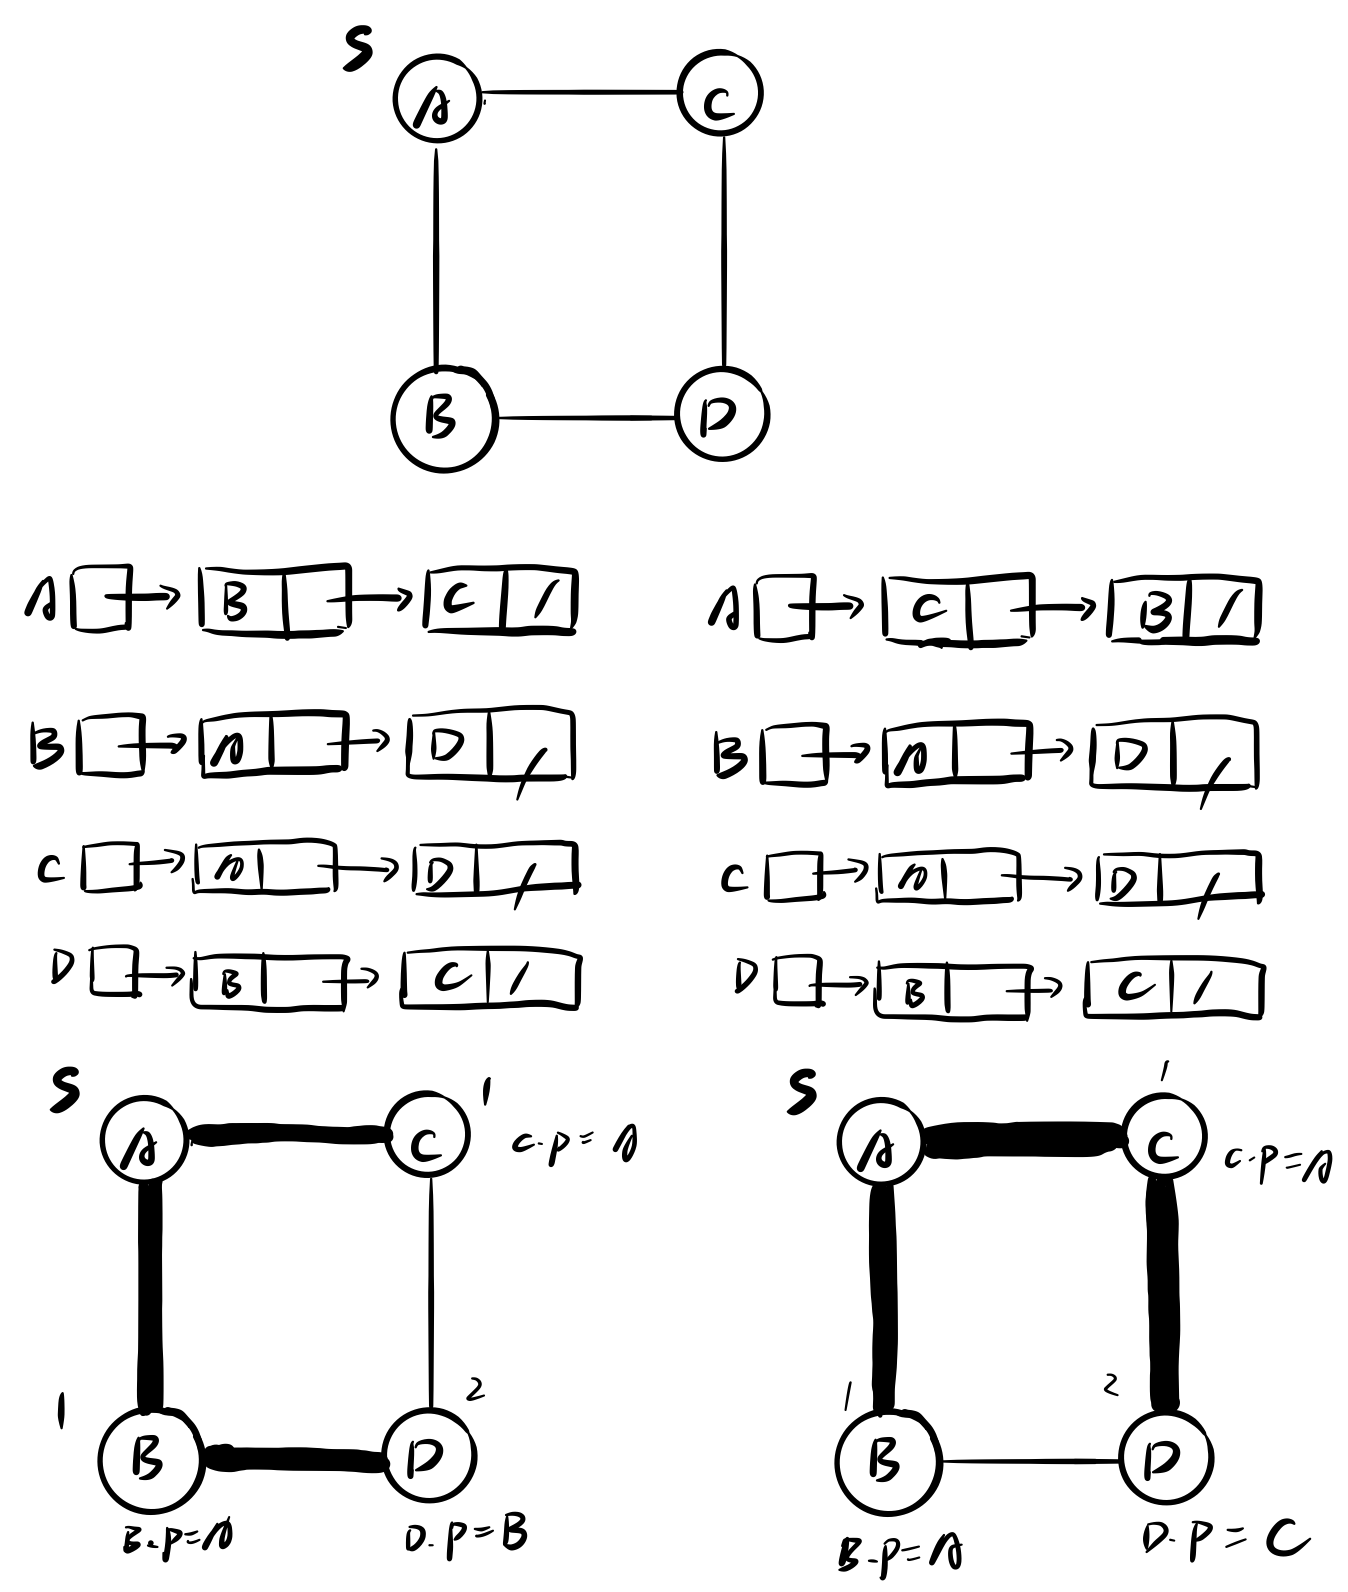
\includegraphics[width=.9\textwidth]{1.png}
	
	Suppose the source vertex is $A$,\ for adjacency lists of different ordering,\ the breadth-first tree is different since $D.p = B$ in the left tree while $D.p = C$ in the right one.
	
	\textbf{(b)}\ The graph is shown below
	
	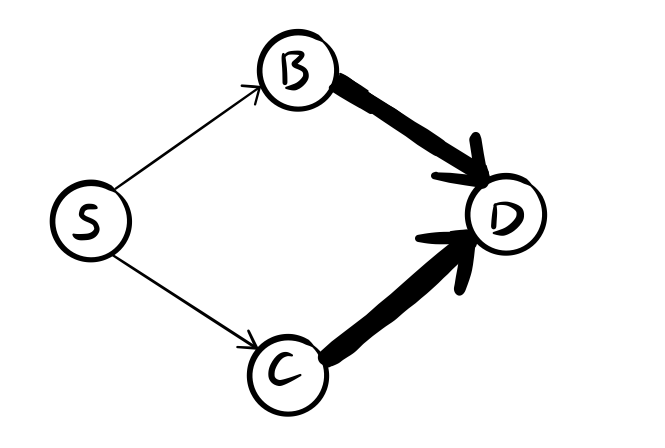
\includegraphics[width=.5\textwidth]{2.png}
	
	No matter $B$ precedes $C$ or $C$ precedes $B$ in the adjacency list $Adj[s]$,\ one of the two bold edges will not be produced.
	
	\section{Problem 5}
	\textbf{(a)}\ The discovery and finishing time is marked near each vertex and the tree edges are bold,\ back edges are $B$,\ forward edges are $F$,\ cross edges are $C$.
	
	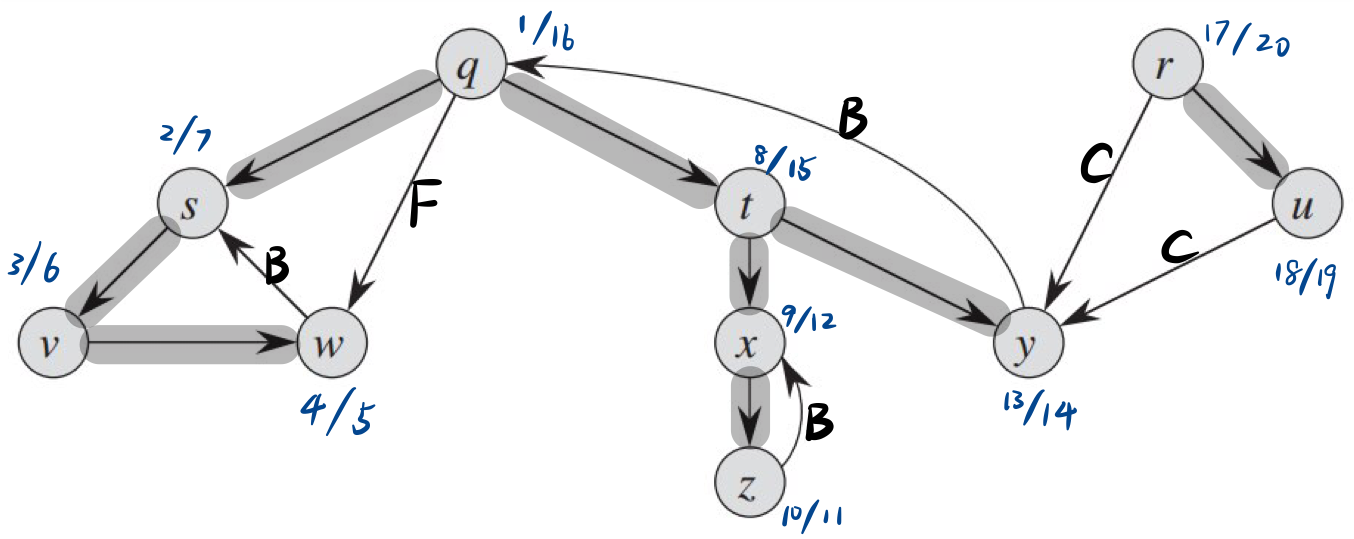
\includegraphics[width=.9\textwidth]{3.png} 
	
	\textbf{(b)}\ A counterexample is given in the folowing

    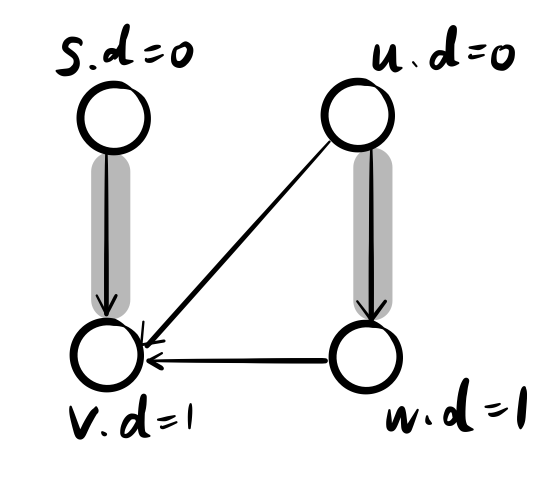
\includegraphics[width=.5\textwidth]{4.png}
    
    Assume the DFS procedures the vertices in alphabetical order,\ we can find that $u.d = 0 < v.d = 1$,\ and graph $G$ contains a path from $u$ to $v$.\ However,\ $v$ is not a descendant of $u$ since the edge $(u,v)$ is a cross edge.
	
	\section{Problem 6}
	\begin{algorithm}[H]
		\caption{DFS(G,s)} % 名称
		\begin{algorithmic}[1]
			\State{$time = time + 1$}
			\State{$s.d = time$}
			\State{$s.color = GRAY$}
			\For{(each edge $(s,v)$ in E)}
			\If{$v.color == BLACK$}
			\If{$v.d > s.d$}
			\State{print $(s,v)$ is forward edge}
			\Else
			\State{print $(s,v)$ is cross edge}
			\EndIf
			\ElsIf{$v.color == GRAY$}
			\State{print $(s,v)$ is back edge}
			\Else
			\State{$DFS(G,v)$}
			\EndIf
			\EndFor
			\State{$s.color = BLACK$}
			\State{$time = time + 1$}
			\State{$s.f = time$}
		\end{algorithmic}
	\end{algorithm}

	\section{Problem 7}
	\textbf{(a)}\ Inspired by the concept of implicit graph,\ we can build a new graph to solve the problem.
	
	Suppose the origin directed graph is $G = (V,E)$,\ we make three copies $V_0$,\ $V_1$,\ $V_2$ of the vertices.\ For each edge $(u,v)\in E$ in the origin graph,\ we create new edges $(u_i,v_j)$ in the new graph where $u_i$ is the corresponding vertex of $u$ in $V_i$,\ $v_j$ is the corresponding vertex of $v$ in $V_j$ and $j = (i+1)\ mod\ 3\ (i=0,1,2)$.\ i.e.\ each edge $(u,v)$ has three corresponding edges $(u_0,v_1),\ (u_1,v_2),\ (u_2,v_0)$ in the new graph.
 
 	Then we comes to the problem.\ Given two vertices $s^0$ and $s^k$ in the origin graph $G$ and a path connected them of length $k$,\ assume all vertices along the path is $s^0,\ s^1\, \cdots, s^{k-1},\ s^k$,\ and the corresponding vertices in the new graph is $s^0_m,\ s^1_{(m+1)\ mod\ 3},\ \cdots,\ s^k_n$.\ Obviously,\ $n = (m+k)\ mod\ 3$.\ If $k$ is divisible by $3$,\ then $n = m$.\ Samely,\ we can prove the inverse proposition is true as well.
 	
 	Deduce from the above proposition,\ if there exists a path from $s_m$ to $t_m$,(e.g.\ $s_0$ and $t_0$) in the new graph,\ which can be implement by BFS,\ then there must exist a walk from $s$ to $t$ whose length is divisible by $3$ in the origin graph,\ and the algorithm will return $\mathtt{true}$.
	
	
\end{document}